% \documentclass{beamer}
\documentclass[hyperref={unicode}]{beamer}

\usepackage{amsmath}
\usepackage{amssymb}
\usepackage{array}
\usepackage{booktabs}
\usepackage{cancel}
\usepackage{color}
\usepackage{datetime2}
\usepackage{textcomp}
\usepackage{gensymb}
\usepackage{graphicx}
\usepackage{mathdots}
\usepackage{multirow}
\usepackage[numbers]{natbib}
\usepackage{pgfplots}
\usepackage{siunitx}
\usepackage{tabularx}
\usepackage{tikz}
\usepackage{yhmath}
\usepackage{hyperref}

\DeclareMathOperator{\Ima}{Im}
\DeclareMathOperator{\Ker}{Ker}
\DeclareMathOperator{\nul}{Null}
\newcommand*{\Z}{\mathbb{Z}}

\usetikzlibrary{fadings}
\usetikzlibrary{patterns}
\usetikzlibrary{shadows.blur}
\usetikzlibrary{arrows}
\usetikzlibrary{decorations.markings}
\usetikzlibrary{positioning}

\pgfplotsset{compat=1.16}

\DTMnewdatestyle{mydateformat}{%
  \renewcommand{\DTMdisplaydate}[4]{%
    \number##1\ % year
    \DTMenglishmonthname{##2}\ % Month
    \number##3% day
  }%
  \renewcommand{\DTMDisplaydate}{\DTMdisplaydate}%
}
\DTMsetdatestyle{mydateformat}

\bibliographystyle{amsalpha}

\usefonttheme[onlymath]{serif}
\usetheme{Darmstadt}
\usecolortheme[RGB={80,80,80}]{structure}
\beamertemplatenavigationsymbolsempty

\newcommand{\bigslant}[2]{{\raisebox{.2em}{$#1$}\left/\raisebox{-.2em}{$#2$}\right.}}


\title{Persistent Homology}
\subtitle{Computations and Applications}
\author{Stephen Ermshar}
\institute{Walla Walla University}
\date{\DTMDisplaydate{2020}{3}{13}{}}

\begin{document}




\begin{frame}
    \titlepage
\end{frame}

\begin{frame}{Outline}
	\tableofcontents
\end{frame}

\section[Motivation]{Motivation}
\begin{frame}
	\textbf{Goal:} Given a collection of points in \(n\)-dimensional space, we want to reveal qualitative properties of an underlying shape that the points may have been sampled from.

	\begin{figure}
		\tikzset{every picture/.style={line width=0.75pt}} %set default line width to 0.75pt

\begin{tikzpicture}[x=0.75pt,y=0.75pt,yscale=-0.5,xscale=0.5]
    \begin{scope}[shift={(-200,0)}]
        \begin{axis}[
            axis line style={draw=none},
            tick style={draw=none},
            yticklabels={,,},
            xticklabels={,,}
        ]
        \addplot table [scatter, only marks, x=x, y=y, col sep=comma] {l23k29-data.csv};
        \end{axis}
    \end{scope}

    \draw[->] (100, 100) -- (150, 100);

    \begin{scope}[shift={(-120,-40)}]
        \draw  [draw opacity=0][fill={rgb, 255:red, 74; green, 144; blue, 226 }  ,fill opacity=1 ,even odd rule] (357,153.5) .. controls (357,121.19) and (383.19,95) .. (415.5,95) .. controls (447.81,95) and (474,121.19) .. (474,153.5) .. controls (474,185.81) and (447.81,212) .. (415.5,212) .. controls (383.19,212) and (357,185.81) .. (357,153.5)(329,153.5) .. controls (329,105.73) and (367.73,67) .. (415.5,67) .. controls (463.27,67) and (502,105.73) .. (502,153.5) .. controls (502,201.27) and (463.27,240) .. (415.5,240) .. controls (367.73,240) and (329,201.27) .. (329,153.5) ;
    \end{scope}
\end{tikzpicture}

		\caption{Motivation Example}
	\end{figure}
	% As a preview, we're going to use these points to construct an object that we can do calculations on, and then we're going to look at how that object changes and doesn't change at different resolutions to see what parts are the most important.
	% before we look at exactly how we construct this object we'll look at how to do the calculations on it.
\end{frame}

\section[Homology]{Homology}
\subsection{Simplicial Homology}
\begin{frame}
	\begin{definition}
		An oriented \textbf{\(n\)-Simplex} will be represented as an \(n\)-tuple of vertices.
	\end{definition}
	\begin{figure}
		\tikzset{every picture/.style={line width=0.75pt}} %set default line width to 0.75pt

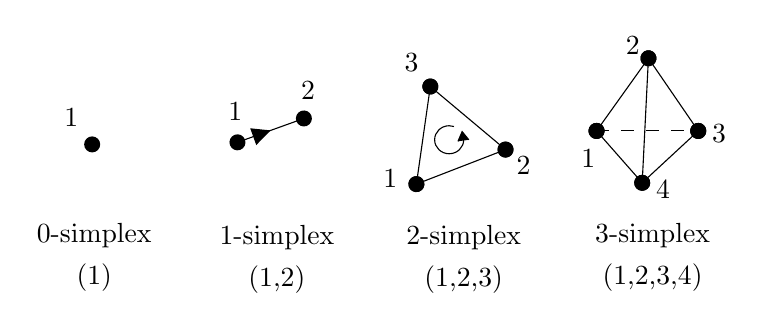
\begin{tikzpicture}[x=0.75pt,y=0.75pt,yscale=-1,xscale=1]
%uncomment if require: \path (0,300); %set diagram left start at 0, and has height of 300

%Straight Lines [id:da29555484994307313]
\draw    (77,72) ;
\draw [shift={(77,72)}, rotate = 0] [color={rgb, 255:red, 0; green, 0; blue, 0 }  ][fill={rgb, 255:red, 0; green, 0; blue, 0 }  ][line width=0.75]      (0, 0) circle [x radius= 3.35, y radius= 3.35]   ;
%Straight Lines [id:da8049693060817193]
\draw    (147,71) -- (179,59.5) ;
\draw [shift={(179,59.5)}, rotate = 340.23] [color={rgb, 255:red, 0; green, 0; blue, 0 }  ][fill={rgb, 255:red, 0; green, 0; blue, 0 }  ][line width=0.75]      (0, 0) circle [x radius= 3.35, y radius= 3.35]   ;
\draw [shift={(163,65.25)}, rotate = 520.23] [fill={rgb, 255:red, 0; green, 0; blue, 0 }  ][line width=0.08]  [draw opacity=0] (8.93,-4.29) -- (0,0) -- (8.93,4.29) -- cycle    ;
\draw [shift={(147,71)}, rotate = 340.23] [color={rgb, 255:red, 0; green, 0; blue, 0 }  ][fill={rgb, 255:red, 0; green, 0; blue, 0 }  ][line width=0.75]      (0, 0) circle [x radius= 3.35, y radius= 3.35]   ;
%Straight Lines [id:da49964849369277564]
\draw    (233.21,91.12) -- (276.15,74.49) ;
\draw [shift={(276.15,74.49)}, rotate = 338.83] [color={rgb, 255:red, 0; green, 0; blue, 0 }  ][fill={rgb, 255:red, 0; green, 0; blue, 0 }  ][line width=0.75]      (0, 0) circle [x radius= 3.35, y radius= 3.35]   ;
\draw [shift={(233.21,91.12)}, rotate = 338.83] [color={rgb, 255:red, 0; green, 0; blue, 0 }  ][fill={rgb, 255:red, 0; green, 0; blue, 0 }  ][line width=0.75]      (0, 0) circle [x radius= 3.35, y radius= 3.35]   ;
%Straight Lines [id:da4902587597827208]
\draw    (239.92,44.11) -- (276.15,74.49) ;
\draw [shift={(276.15,74.49)}, rotate = 39.97] [color={rgb, 255:red, 0; green, 0; blue, 0 }  ][fill={rgb, 255:red, 0; green, 0; blue, 0 }  ][line width=0.75]      (0, 0) circle [x radius= 3.35, y radius= 3.35]   ;
\draw [shift={(239.92,44.11)}, rotate = 39.97] [color={rgb, 255:red, 0; green, 0; blue, 0 }  ][fill={rgb, 255:red, 0; green, 0; blue, 0 }  ][line width=0.75]      (0, 0) circle [x radius= 3.35, y radius= 3.35]   ;
%Straight Lines [id:da706097538890246]
\draw    (233.21,91.12) -- (239.92,44.11) ;
\draw [shift={(239.92,44.11)}, rotate = 278.12] [color={rgb, 255:red, 0; green, 0; blue, 0 }  ][fill={rgb, 255:red, 0; green, 0; blue, 0 }  ][line width=0.75]      (0, 0) circle [x radius= 3.35, y radius= 3.35]   ;
\draw [shift={(233.21,91.12)}, rotate = 278.12] [color={rgb, 255:red, 0; green, 0; blue, 0 }  ][fill={rgb, 255:red, 0; green, 0; blue, 0 }  ][line width=0.75]      (0, 0) circle [x radius= 3.35, y radius= 3.35]   ;
%Straight Lines [id:da26537918293179197]
\draw    (342,90.5) -- (369,65.5) ;
\draw [shift={(369,65.5)}, rotate = 317.2] [color={rgb, 255:red, 0; green, 0; blue, 0 }  ][fill={rgb, 255:red, 0; green, 0; blue, 0 }  ][line width=0.75]      (0, 0) circle [x radius= 3.35, y radius= 3.35]   ;
\draw [shift={(342,90.5)}, rotate = 317.2] [color={rgb, 255:red, 0; green, 0; blue, 0 }  ][fill={rgb, 255:red, 0; green, 0; blue, 0 }  ][line width=0.75]      (0, 0) circle [x radius= 3.35, y radius= 3.35]   ;
%Straight Lines [id:da6451030111536471]
\draw  [dash pattern={on 4.5pt off 4.5pt}]  (320,65.5) -- (369,65.5) ;
\draw [shift={(369,65.5)}, rotate = 0] [color={rgb, 255:red, 0; green, 0; blue, 0 }  ][fill={rgb, 255:red, 0; green, 0; blue, 0 }  ][line width=0.75]      (0, 0) circle [x radius= 3.35, y radius= 3.35]   ;
\draw [shift={(320,65.5)}, rotate = 0] [color={rgb, 255:red, 0; green, 0; blue, 0 }  ][fill={rgb, 255:red, 0; green, 0; blue, 0 }  ][line width=0.75]      (0, 0) circle [x radius= 3.35, y radius= 3.35]   ;
%Straight Lines [id:da5075115445773606]
\draw    (342,90.5) -- (320,65.5) ;
\draw [shift={(320,65.5)}, rotate = 228.65] [color={rgb, 255:red, 0; green, 0; blue, 0 }  ][fill={rgb, 255:red, 0; green, 0; blue, 0 }  ][line width=0.75]      (0, 0) circle [x radius= 3.35, y radius= 3.35]   ;
\draw [shift={(342,90.5)}, rotate = 228.65] [color={rgb, 255:red, 0; green, 0; blue, 0 }  ][fill={rgb, 255:red, 0; green, 0; blue, 0 }  ][line width=0.75]      (0, 0) circle [x radius= 3.35, y radius= 3.35]   ;
%Straight Lines [id:da7438166459098603]
\draw    (320,65.5) -- (345,30.5) ;
\draw [shift={(345,30.5)}, rotate = 305.54] [color={rgb, 255:red, 0; green, 0; blue, 0 }  ][fill={rgb, 255:red, 0; green, 0; blue, 0 }  ][line width=0.75]      (0, 0) circle [x radius= 3.35, y radius= 3.35]   ;
\draw [shift={(320,65.5)}, rotate = 305.54] [color={rgb, 255:red, 0; green, 0; blue, 0 }  ][fill={rgb, 255:red, 0; green, 0; blue, 0 }  ][line width=0.75]      (0, 0) circle [x radius= 3.35, y radius= 3.35]   ;
%Straight Lines [id:da7652267815198734]
\draw    (369,65.5) -- (345,30.5) ;
\draw [shift={(345,30.5)}, rotate = 235.56] [color={rgb, 255:red, 0; green, 0; blue, 0 }  ][fill={rgb, 255:red, 0; green, 0; blue, 0 }  ][line width=0.75]      (0, 0) circle [x radius= 3.35, y radius= 3.35]   ;
\draw [shift={(369,65.5)}, rotate = 235.56] [color={rgb, 255:red, 0; green, 0; blue, 0 }  ][fill={rgb, 255:red, 0; green, 0; blue, 0 }  ][line width=0.75]      (0, 0) circle [x radius= 3.35, y radius= 3.35]   ;
%Straight Lines [id:da555816554232639]
\draw    (345,30.5) -- (342,90.5) ;
%Shape: Arc [id:dp712681679883792]
\draw  [draw opacity=0] (255.97,69.08) .. controls (255.99,69.3) and (256,69.52) .. (256,69.75) .. controls (256,73.48) and (252.87,76.5) .. (249,76.5) .. controls (245.13,76.5) and (242,73.48) .. (242,69.75) .. controls (242,66.02) and (245.13,63) .. (249,63) .. controls (249.81,63) and (250.59,63.13) .. (251.32,63.38) -- (249,69.75) -- cycle ; \draw   (255.97,69.08) .. controls (255.99,69.3) and (256,69.52) .. (256,69.75) .. controls (256,73.48) and (252.87,76.5) .. (249,76.5) .. controls (245.13,76.5) and (242,73.48) .. (242,69.75) .. controls (242,66.02) and (245.13,63) .. (249,63) .. controls (249.81,63) and (250.59,63.13) .. (251.32,63.38) ;
\draw  [fill={rgb, 255:red, 0; green, 0; blue, 0 }  ,fill opacity=1 ] (253.25,70.52) -- (255.25,65.85) -- (258.47,69.77) ;

% Text Node
\draw (78,116) node   [align=left] {0-simplex};
% Text Node
\draw (166,117) node   [align=left] {1-simplex};
% Text Node
\draw (256,117) node   [align=left] {2-simplex};
% Text Node
\draw (347,116) node   [align=left] {3-simplex};
% Text Node
\draw (78,136) node   [align=left] {(1)};
% Text Node
\draw (166,137) node   [align=left] {(1,2)};
% Text Node
\draw (256,137) node   [align=left] {(1,2,3)};
% Text Node
\draw (347,136) node   [align=left] {(1,2,3,4)};
% Text Node
\draw (67,59) node   [align=left] {1};
% Text Node
\draw (146,56) node   [align=left] {1};
% Text Node
\draw (181,46) node   [align=left] {2};
% Text Node
\draw (220.6,88.23) node   [align=left] {1};
% Text Node
\draw (284.84,82.27) node   [align=left] {2};
% Text Node
\draw (230.91,32.78) node   [align=left] {3};
% Text Node
\draw (316,79) node   [align=left] {1};
% Text Node
\draw (337.5,24.5) node   [align=left] {2};
% Text Node
\draw (379,67) node   [align=left] {3};
% Text Node
\draw (352,94) node   [align=left] {4};


\end{tikzpicture}

		\caption{Examples of basic simplices.}
	\end{figure}
\end{frame}

\begin{frame}
	\begin{definition}
		A \textbf{Simplicial Complex} is a finite collection of finite sets such that every subset of every element in the collection is also an element in the collection. \cite{wagner}
	\end{definition}
	\begin{figure}
		\tikzset{every picture/.style={line width=0.75pt}} %set default line width to 0.75pt

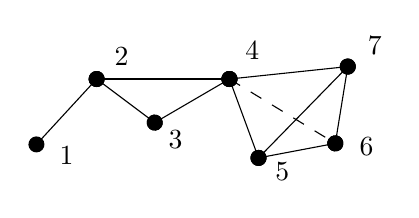
\begin{tikzpicture}[x=0.75pt,y=0.75pt,yscale=-1,xscale=1]
%uncomment if require: \path (0,95); %set diagram left start at 0, and has height of 95

%Straight Lines [id:da20686486428426965]
\draw    (13,61) -- (42,29.5) ;
\draw [shift={(42,29.5)}, rotate = 312.63] [color={rgb, 255:red, 0; green, 0; blue, 0 }  ][fill={rgb, 255:red, 0; green, 0; blue, 0 }  ][line width=0.75]      (0, 0) circle [x radius= 3.35, y radius= 3.35]   ;
\draw [shift={(13,61)}, rotate = 312.63] [color={rgb, 255:red, 0; green, 0; blue, 0 }  ][fill={rgb, 255:red, 0; green, 0; blue, 0 }  ][line width=0.75]      (0, 0) circle [x radius= 3.35, y radius= 3.35]   ;
%Straight Lines [id:da9899744043809231]
\draw    (42,29.5) -- (106,29.5) ;
\draw [shift={(106,29.5)}, rotate = 0] [color={rgb, 255:red, 0; green, 0; blue, 0 }  ][fill={rgb, 255:red, 0; green, 0; blue, 0 }  ][line width=0.75]      (0, 0) circle [x radius= 3.35, y radius= 3.35]   ;
\draw [shift={(42,29.5)}, rotate = 0] [color={rgb, 255:red, 0; green, 0; blue, 0 }  ][fill={rgb, 255:red, 0; green, 0; blue, 0 }  ][line width=0.75]      (0, 0) circle [x radius= 3.35, y radius= 3.35]   ;
%Straight Lines [id:da4483952202454973]
\draw    (42,29.5) -- (70,50.5) ;
\draw [shift={(70,50.5)}, rotate = 36.87] [color={rgb, 255:red, 0; green, 0; blue, 0 }  ][fill={rgb, 255:red, 0; green, 0; blue, 0 }  ][line width=0.75]      (0, 0) circle [x radius= 3.35, y radius= 3.35]   ;
\draw [shift={(42,29.5)}, rotate = 36.87] [color={rgb, 255:red, 0; green, 0; blue, 0 }  ][fill={rgb, 255:red, 0; green, 0; blue, 0 }  ][line width=0.75]      (0, 0) circle [x radius= 3.35, y radius= 3.35]   ;
%Straight Lines [id:da013663715151336797]
\draw    (70,50.5) -- (106,29.5) ;
\draw [shift={(106,29.5)}, rotate = 329.74] [color={rgb, 255:red, 0; green, 0; blue, 0 }  ][fill={rgb, 255:red, 0; green, 0; blue, 0 }  ][line width=0.75]      (0, 0) circle [x radius= 3.35, y radius= 3.35]   ;
\draw [shift={(70,50.5)}, rotate = 329.74] [color={rgb, 255:red, 0; green, 0; blue, 0 }  ][fill={rgb, 255:red, 0; green, 0; blue, 0 }  ][line width=0.75]      (0, 0) circle [x radius= 3.35, y radius= 3.35]   ;
%Straight Lines [id:da6445202628566384]
\draw    (106,29.5) -- (163,23.5) ;
\draw [shift={(163,23.5)}, rotate = 353.99] [color={rgb, 255:red, 0; green, 0; blue, 0 }  ][fill={rgb, 255:red, 0; green, 0; blue, 0 }  ][line width=0.75]      (0, 0) circle [x radius= 3.35, y radius= 3.35]   ;
\draw [shift={(106,29.5)}, rotate = 353.99] [color={rgb, 255:red, 0; green, 0; blue, 0 }  ][fill={rgb, 255:red, 0; green, 0; blue, 0 }  ][line width=0.75]      (0, 0) circle [x radius= 3.35, y radius= 3.35]   ;
%Straight Lines [id:da3743946516627876]
\draw    (106,29.5) -- (120,67.5) ;
\draw [shift={(120,67.5)}, rotate = 69.78] [color={rgb, 255:red, 0; green, 0; blue, 0 }  ][fill={rgb, 255:red, 0; green, 0; blue, 0 }  ][line width=0.75]      (0, 0) circle [x radius= 3.35, y radius= 3.35]   ;
\draw [shift={(106,29.5)}, rotate = 69.78] [color={rgb, 255:red, 0; green, 0; blue, 0 }  ][fill={rgb, 255:red, 0; green, 0; blue, 0 }  ][line width=0.75]      (0, 0) circle [x radius= 3.35, y radius= 3.35]   ;
%Straight Lines [id:da2401873796980163]
\draw    (120,67.5) -- (163,23.5) ;
\draw [shift={(163,23.5)}, rotate = 314.34] [color={rgb, 255:red, 0; green, 0; blue, 0 }  ][fill={rgb, 255:red, 0; green, 0; blue, 0 }  ][line width=0.75]      (0, 0) circle [x radius= 3.35, y radius= 3.35]   ;
\draw [shift={(120,67.5)}, rotate = 314.34] [color={rgb, 255:red, 0; green, 0; blue, 0 }  ][fill={rgb, 255:red, 0; green, 0; blue, 0 }  ][line width=0.75]      (0, 0) circle [x radius= 3.35, y radius= 3.35]   ;
%Straight Lines [id:da08347218855288774]
\draw  [dash pattern={on 4.5pt off 4.5pt}]  (106,29.5) -- (157,60.5) ;
\draw [shift={(157,60.5)}, rotate = 31.29] [color={rgb, 255:red, 0; green, 0; blue, 0 }  ][fill={rgb, 255:red, 0; green, 0; blue, 0 }  ][line width=0.75]      (0, 0) circle [x radius= 3.35, y radius= 3.35]   ;
\draw [shift={(106,29.5)}, rotate = 31.29] [color={rgb, 255:red, 0; green, 0; blue, 0 }  ][fill={rgb, 255:red, 0; green, 0; blue, 0 }  ][line width=0.75]      (0, 0) circle [x radius= 3.35, y radius= 3.35]   ;
%Straight Lines [id:da34695654406224863]
\draw    (120,67.5) -- (157,60.5) ;
\draw [shift={(157,60.5)}, rotate = 349.29] [color={rgb, 255:red, 0; green, 0; blue, 0 }  ][fill={rgb, 255:red, 0; green, 0; blue, 0 }  ][line width=0.75]      (0, 0) circle [x radius= 3.35, y radius= 3.35]   ;
\draw [shift={(120,67.5)}, rotate = 349.29] [color={rgb, 255:red, 0; green, 0; blue, 0 }  ][fill={rgb, 255:red, 0; green, 0; blue, 0 }  ][line width=0.75]      (0, 0) circle [x radius= 3.35, y radius= 3.35]   ;
%Straight Lines [id:da5097015872445443]
\draw    (163,23.5) -- (157,60.5) ;
\draw [shift={(157,60.5)}, rotate = 99.21] [color={rgb, 255:red, 0; green, 0; blue, 0 }  ][fill={rgb, 255:red, 0; green, 0; blue, 0 }  ][line width=0.75]      (0, 0) circle [x radius= 3.35, y radius= 3.35]   ;
\draw [shift={(163,23.5)}, rotate = 99.21] [color={rgb, 255:red, 0; green, 0; blue, 0 }  ][fill={rgb, 255:red, 0; green, 0; blue, 0 }  ][line width=0.75]      (0, 0) circle [x radius= 3.35, y radius= 3.35]   ;


% Text Node
\draw (27.5,66.5) node    {$1$};
% Text Node
\draw (54,18.5) node    {$2$};
% Text Node
\draw (80,58.5) node    {$3$};
% Text Node
\draw (117,16) node    {$4$};
% Text Node
\draw (131.5,74) node    {$5$};
% Text Node
\draw (172,62) node    {$6$};
% Text Node
\draw (176,13.5) node    {$7$};


\end{tikzpicture}

		\caption{Example simplicial complex with two connected components, one hole, and one void.}
	\end{figure}
	\begin{align*}
		S = \{
			&(4,5,7), (5,6,7), (4,6,7), (4,5,6),\quad (1,2), (2,3),\\ &(3,4), (2,4), (4,5), (5,6),(6,7),(4,7),(4,6),(5,7),\\
			&(1), (2), (3), (4), (5), (6), (7), (8)
		\}
	\end{align*}
\end{frame}

\subsection{Computations}
\begin{frame}
	\begin{definition}
		The \textbf{Boundary Homomorphism} is a function that takes a simplex and returns its boundary.
	\end{definition}
\end{frame}


\section[Persistence]{Persistent Homology}
\subsection{\v{C}ech, Rips, and Witness Complexes}
\begin{frame}
\end{frame}

\section{Applications}
\subsection{Visualization and Compression}
\begin{frame}
\end{frame}

\section*{Bibliography}
\begin{frame}{Bibliography}
	\nocite{wagner}
	\nocite{hatcher}
	\nocite{fraleigha}
	\nocite{singh}
	% https://tex.stackexchange.com/a/22654
	\begingroup
	\renewcommand{\section}[2]{}%
	\bibliography{../math496-7-zotero.bib}
	\endgroup
\end{frame}




\end{document}
